\section{Assessment for operational safety}
\label{sec:assessment}

This section describes shortly the steps of the M3 assessment, an assessment for the operational safety of an autonomous vehicle (AV). 
We will also describe the use of testing in the assessment and the procedure of the M3 assessment.


\subsection{Steps of the assessment}

The assessment procedure is schematically shown in \cref{fig:assessment activities} using the yellow blocks. Furthermore, \cref{fig:assessment activities} shows the four aspects of operational safety which were described in \cref{sec:safety}. The arrows between the aspects of operational safety and the different activities of the assessment procedure indicate what the focus is of the activities.  

Before  starting the assessment of an AV, the AV developer needs to apply for the assessment through the application procedure. With the application for the assessment, the AV developer needs to declare a vehicle deployment specification to describe the vehicle, how it is operated and where it is expected to be able to operate according to specifications. 
%For more details of the application, see \cref{sec:application}.

%Describe shortly how the assessment procedure looks like, see \cref{fig:assessment activities}. Explain how the different steps relate to the different aspects of operational safety.

% Document review
The first step of the actual assessment procedure is the document review. This is an important tool for determining whether the procedures of the AV developer comply with the functional safety requirements according to ISO~26262 or the developer's own policies and procedures regarding functional safety comparable to ISO~26262. Furthermore, the document review enables assessing whether the developer has a sufficiently developed process for managing cybersecurity across their organisation and all systems involved in the deployment. 
%More details on the document review are presented in \cref{sec:document review}.

% Lab tests for cyber security
The lab tests for the cybersecurity assessment is a physical inspection and observation procedure. The aim is to check that the systems are as described in the cybersecurity relevant documentation provided for document review, review/detect physical and access related vulnerabilities, review service procedure access and controls, and demonstrate the monitoring systems used for detecting potential attacks. 

% Tests for fail safety
Similarly, also tests for the AV to exhibit fail safe behaviour are performed following the document review. The document review reveals the ODD for which the AV is designed, and based on this information reasonably straightforward tests are selected to check the response of the AV when forced to cross the border of the ODD. Moreover, checks are performed regarding the response of the vehicle to malfunction of sensors or physical control component damage. Also the secondary fallback system (e.g., takeover of the control by the monitoring safety driver) needs to be checked in this step of the assessment procedure. 

% Simulations
Virtual testing allows a wide range of test cases (e.g. from normal every day driving cases to critical test cases) to be executed safely in a virtual environment. In this step of the assessment, the simulation results provided by the AV developers are reviewed. The results for the relevant test cases are compared to the expected results based on \textit{a priori} selected KPIs and a safety rating is provided based on virtual results only. The analysis of results will provide input for the selection of a limited number of test cases that are tested physically.

%Physical tests
Physical tests serve a twofold purpose. At one hand the results of physical tests are directly used as input for the assessment of safety. On the other hand, results are used to validate the simulations that are used in the evaluation. In the review of the simulation results, the assessors will make a selection of test cases that need to be performed as a physical test for simulation validation. The results of the physical test prevail over the results of the simulation for the same test case. Physical tests are not limited to simulation validation. Also \textit{a priori} selected test cases are used for assessing the safety of the vehicle. The test cases for the virtual and physical tests together should be reasonably distributed over the ODD of the AV. 

%Road tests
Once the physical and virtual assessment has passed successfully, an on-road test is used to check the readiness of the AV to be deployed on the road. A customized route for each AV is driven based on its ODD. Again, the test results are validated using pass/fail criteria. As no fixed well-specified scenarios are expected, the evaluation is similar to the traffic police assessment of drivers that apply for a driving license. The road tests are performed with a safety driver and assessor on board. The safety driver needs to take-over control the moment a situation turns out to become unsafe. In an \textit{a posteriori} evaluation it will be decided whether the AV has passed the test or not.


\begin{figure*}
	\centering
	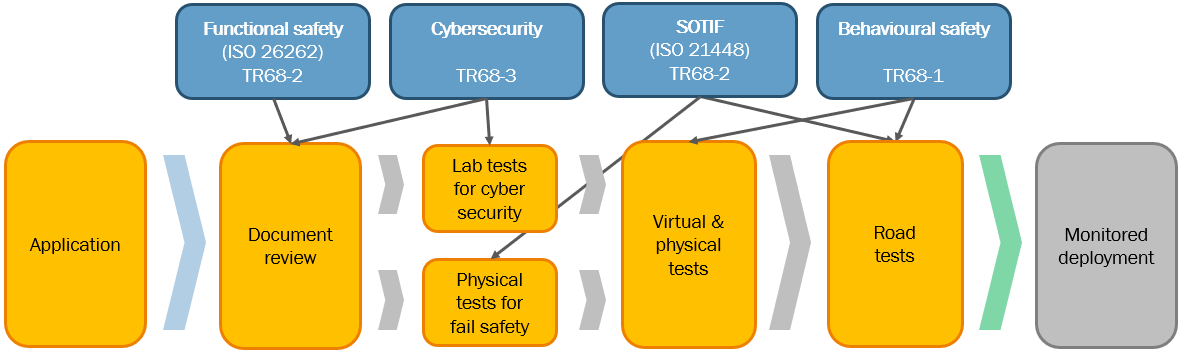
\includegraphics[width=\linewidth]{assessment_activities}
	\caption{Overview of the assessment activities in yellow.}
	\label{fig:assessment activities}
\end{figure*}



\todo{Go into a bit more details on the different blocks of \cref{fig:assessment activities}. Perhaps a subsection for each block.}


%\subsection{Testing}
%\label{sec:use of testing}
%
%%\subsubsection{Process of test definition}
%Following the IEEE definition of the notion of \emph{test} \cite{ieee1990glossary} and clearly explained in \cite{stellet2015taxonomy}, a test consists of the following components:
%\begin{itemize}
%	\item A statement on the system-under-test (\emph{test criteria}, i.e., what we are going to evaluate using the test?);
%	\item A set of specified conditions (\emph{test case}, i.e., how we are going to evaluate the test criteria?);
%	\item Quantitative measures (\emph{metrics}, i.e., how do we express quantitatively the outcome of a test); and
%	\item Knowledge of an ideal result (\emph{reference}, i.e., when is an outcome acceptable?)
%\end{itemize}
%Using these four components, a test can be described as an evaluation of the test criteria quantitatively expressed according to metrics in a test case with a reference.
%
%\Cref{fig:process to test} shows schematically the process for defining the tests and obtaining the test result. The process assumes that a developed AV (function) needs to be evaluated. The design of the AV comes with a range of operating conditions, i.e., the Operational Design Domain (ODD), and the functional requirements. Based on the ODD and the functional requirements, the relevant scenarios or scenario classes can be selected out of the possible scenario classes, see, e.g., \cite{degelder2019scenarioclasses}. The ODD and the functional requirements also form the basis of the test criteria. Based on the relevant scenarios or scenario classes and the test criteria, the test cases are generated. To perform the test, a test plan needs to be designed that describes how the test in the given conditions (described by the test case) is performed. Next, from the actual performed tests, the test results are obtained according to some metrics that are derived from the test criteria. The test results are compared with a reference that is based on the ODD, the functional requirements, and the metrics. If the comparison results in a ``pass'', the next test can be performed until the AV passed the whole assessment. However, if this comparison results in a ``fail'', it means that the design of the AV needs to be reconsidered. Possibly a refining step is required. 
%
%\begin{figure*}
%	\centering
%	% Define colors
\definecolor{colorCETRAN}{RGB}{160, 230, 255}
\definecolor{colorAV}{RGB}{255, 200, 160}
%
% Define lengths
\newlength{\blkw}\setlength{\blkw}{9em}
\newlength{\blkh}\setlength{\blkh}{4em}
\newlength{\sep}\setlength{\sep}{2em}
%
% Define styles
\tikzstyle{block}=[draw, minimum width=\blkw, minimum height=\blkh, text width=\blkw-1em, align=center, anchor=north west, line width=.5pt]
\tikzstyle{assessor}=[block, fill=colorCETRAN]
\tikzstyle{av}=[block, fill=colorAV]
\tikzstyle{assessor and av}=[block, left color=colorCETRAN, right color=colorAV]
\tikzstyle{decision}=[draw, diamond, minimum width=2em, minimum height=3em, line width=1pt]
\tikzstyle{arrow}=[->, line width=2pt]
\begin{tikzpicture}
	% Blocks
	\node[av](design) at (0, 0) {Design AV};
	\node[av, minimum height=3\blkh+2\sep](odd) at (0, -\blkh-\sep) {Describe ODD \& Functional requirements};
	\node[assessor](select) at (0, -4\blkh-4\sep) {Select relevant scenario (classes)};
	\node[assessor](reference) at (\blkw+\sep, -\blkh-\sep) {Determine reference};
	\node[assessor](metrics) at (\blkw+\sep, -2\blkh-2\sep) {Determine metrics};
	\node[assessor](criteria) at (\blkw+\sep, -3\blkh-3\sep) {Define test criteria};
	\node[assessor](test case) at (\blkw+\sep, -4\blkh-4\sep) {Generate test cases};
	\node[assessor](compare) at (2\blkw+2\sep, -\blkh-\sep) {Compare with reference};
	\node[assessor and av, minimum height=2\blkh+\sep](obtain metrics) at (2\blkw+2\sep, -2\blkh-2\sep) {Obtain test results (according to metrics)};
	\node[assessor](test) at (2\blkw+2\sep, -4\blkh-4\sep) {Design test plan};
	
	% Decision block
	\node[decision](decision) at (2.5\blkw+2\sep, -.5\blkh){};
	\node[right of=decision, node distance=\blkw, text width=7em, align=center](next) {Continue with other test};
	
	% Arrows
	\draw[arrow] (design) -- (odd);
	\draw[arrow] (odd) -- (select);
	\foreach \blk in {reference, criteria} {
		\node[coordinate, left of=\blk, node distance=.5\blkw+\sep](helper){};
		\draw[arrow] (helper) -- (\blk);
	}
	\draw[arrow] (metrics) -- (reference);
	\draw[arrow] (criteria) -- (metrics);
	\draw[arrow] (select) -- (test case);
	\draw[arrow] (criteria) -- (test case);
	\draw[arrow] (test case) -- (test);
	\draw[arrow] (test) -- (obtain metrics);
	\node[coordinate, right of=metrics, node distance=.5\blkw+\sep](helper){};
	\draw[arrow] (metrics) -- (helper);
	\draw[arrow] (obtain metrics) -- (compare);
	\draw[arrow] (reference) -- (compare);
	\draw[arrow] (compare) -- (decision);
	\draw[arrow] (decision) -- node[fill=white, align=center, text width=3em]{Refine design} (design);
	\draw[arrow] (decision) -- (next);
\end{tikzpicture}
%	\caption{Schematic overview of the process used for defining tests and obtaining test results. The orange blocks indicate the tasks for which the AV developer is responsible whereas the blue blocks indicate the responsibility of the assessor. Obtaining the test results is the responsibility of both the AV developer and the assessor.}
%	\label{fig:process to test}
%\end{figure*}
%
%The schematic overview in \cref{fig:process to test} shows activities that need to be carried out by both the AV developer and the assessor. Obviously, the AV developer is responsible for the design of the AV. The description of the ODD and the functional requirements is provided to the assessor by the AV developer. Obtaining the test results is done by either the AV developer or the assessor. For example, the virtual simulations are performed by the AV developer. Physical tests are done by both the assessor and the AV developer. For all other activities mentioned in \cref{fig:process to test}, the assessor is responsible. 

%\subsubsection{Test example: pass/fail testing versus grading}
%\label{sec:test example}
%To illustrate a test, let us assume an AV that is required to drive on a straight urban road with a speed of \unit[25]{km/h}. The test criterion could read as ``the AV stays in its lane while driving on a straight urban road keeping a predefined speed matching the local speed regulations''. To test this criterion, one or more test cases need to be considered depending on the ODD and the functional requirements. Also possible variations regarding driving on a straight road need to be considered. Variations might include the number of lanes, only one or two-directional driving, weather conditions, lighting conditions, actors within the AV's lane and/or next to it, the lane markings, the type of road edge, the presence of infrastructural objects, etc.
% 
%\begin{figure}
%	\centering
%	\begin{subfigure}[t]{.8\linewidth}
%		\centering
%		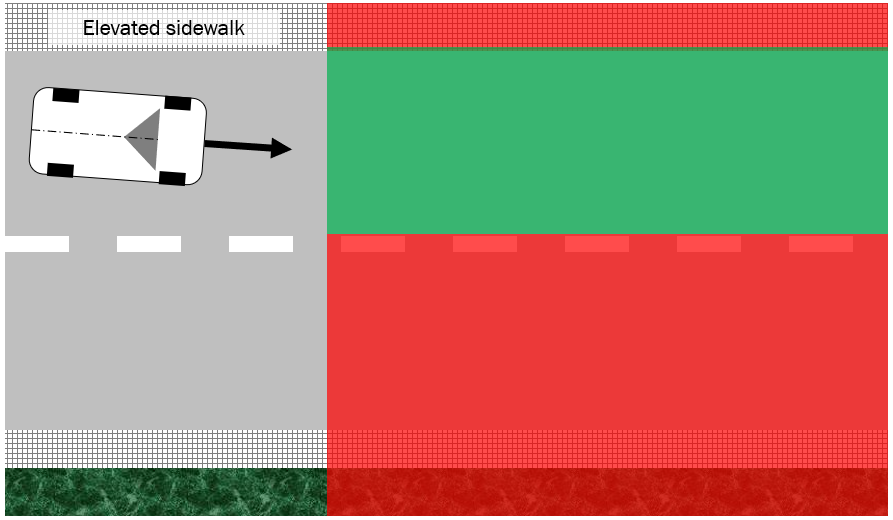
\includegraphics[width=\linewidth]{test_example_failpass}
%		\caption{Binary outcome: a fail when the AV enters the red area.}
%		\label{fig:test example pass fail}
%	\end{subfigure}\\
%	\begin{subfigure}[t]{.98\linewidth}
%		\centering
%		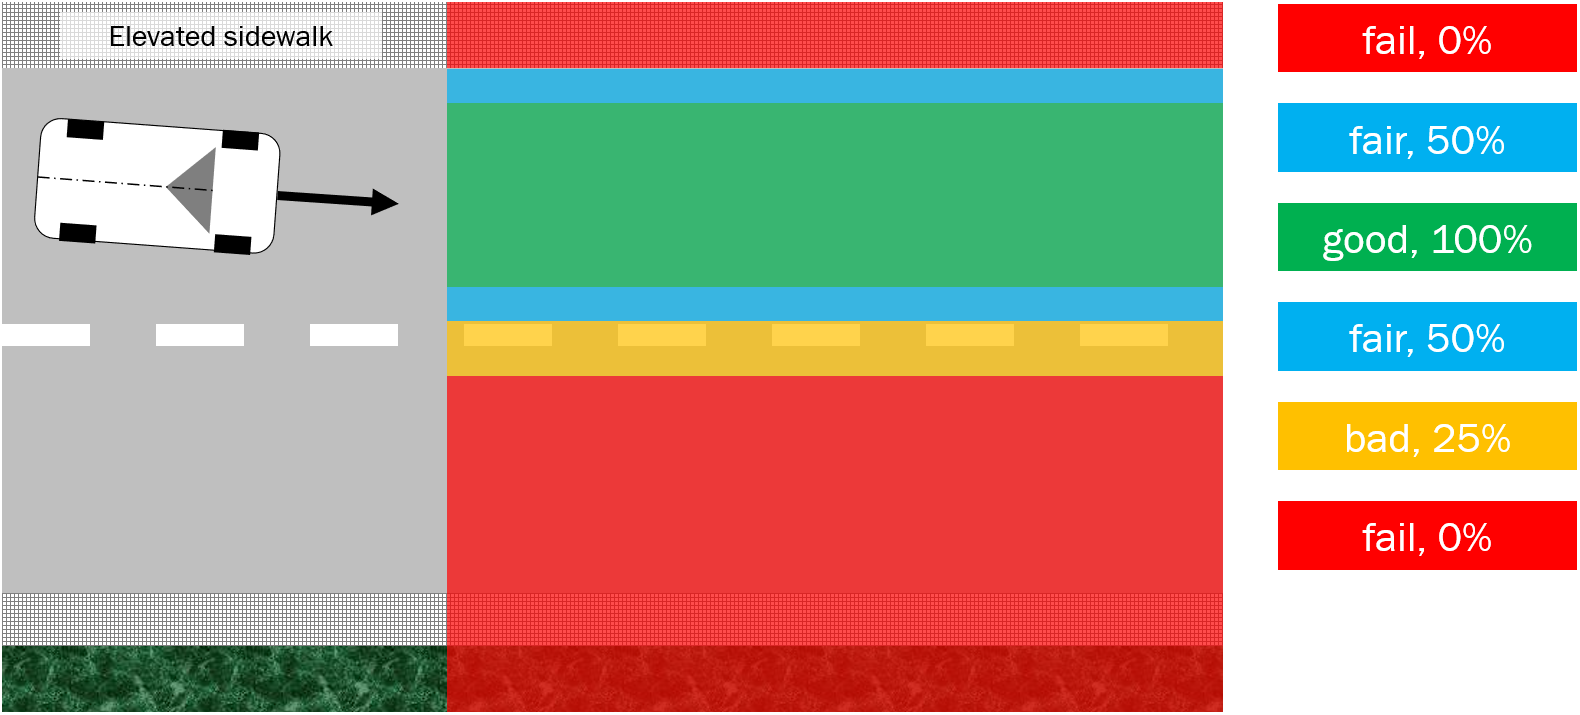
\includegraphics[width=\linewidth]{test_example_failpassvague}
%		\caption{Test where the result is not binary but more graded.}
%		\label{fig:test example pass fail vague}
%	\end{subfigure}
%	\caption{Test where the objective of the Automated Vehicle (AV) is to drive straight on a two lane road.}
%	\label{fig:test example}
%\end{figure}
%
%An example of a test case is shown in \cref{fig:test example pass fail}. Here, the AV drives on a two lane bi-directional road in the left lane. An elevated sidewalk is on the left of the AV. The lanes are divided by a dashed center line marking. To quantify the performance of the AV, appropriate metrics need to be chosen. This could, for example, be the distance of the AV towards the elevated sidewalk and the distance of the AV towards the line markings on the AV's right side. If one of these distances over the course of the test becomes equal to zero, the AV fails the test. This is indicated by the green and red areas in \cref{fig:test example pass fail}. If the vehicle is within the green area during the complete test, the test is passed. In case the vehicle crosses the border between green and red area at any given point in time during the test, the test fails.
%
%\begin{figure}
%	\centering
%	\begin{subfigure}[t]{.46\linewidth}
%		\centering
%		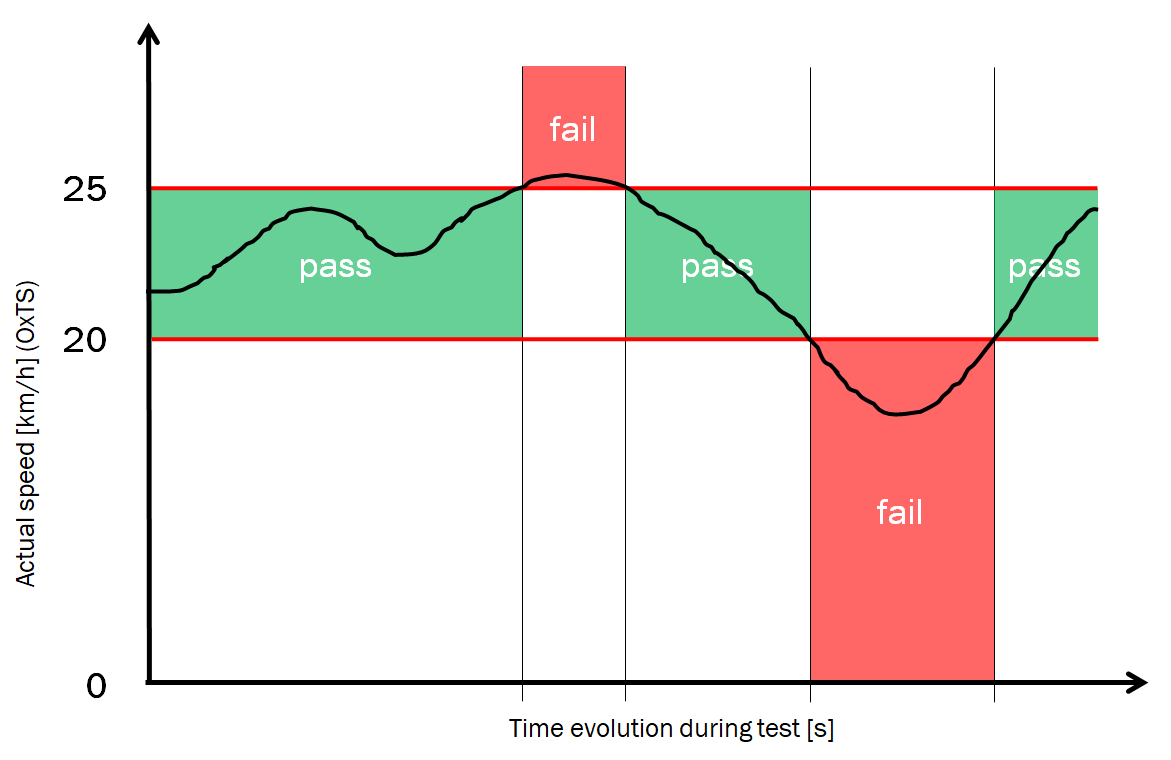
\includegraphics[height=4.5cm]{test_example_speed}
%		\caption{Binary outcome: a fail when the AV speed crosses the bounds of the allowed speed corridor.}
%		\label{fig:test speed pass fail}
%	\end{subfigure} \\
%	\begin{subfigure}[t]{.46\linewidth}
%		\centering
%		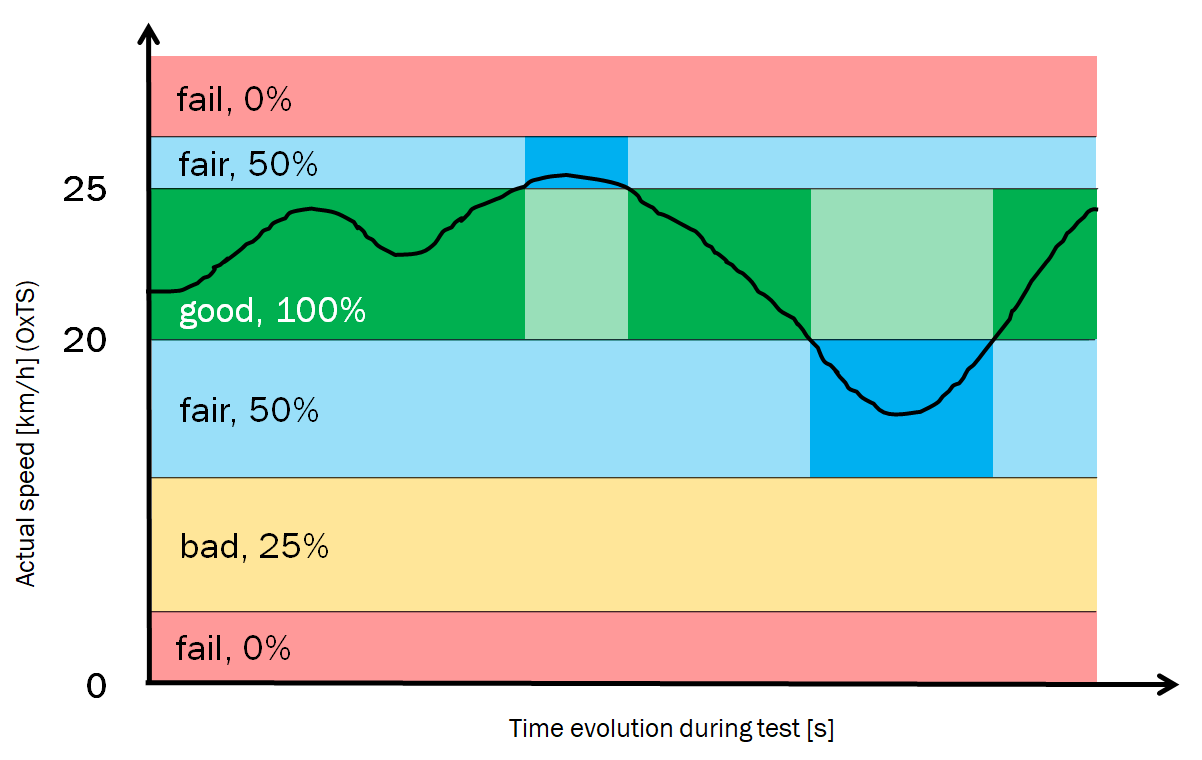
\includegraphics[height=4.5cm]{test_example_speed_grades}
%		\caption{Test where the result is more graded; here the result is fair instead of a fail.}
%		\label{fig:test speed grades}
%	\end{subfigure}
%	\label{fig:test speed}
%	\caption{Test where the objective of the Automated Vehicle (AV) is to show an appropriate speed while driving straight without obstructions.}
%	\label{fig:test example speed}
%\end{figure}
% 
%A variation of the test in \cref{fig:test example pass fail} is shown in \cref{fig:test example pass fail vague}. Whereas the test in \cref{fig:test example pass fail} has a binary outcome (pass or fail), the outcome of the test in \cref{fig:test example pass fail vague} is a score ranging from \unit[0]{\%} to \unit[100]{\%}. The score is calculated during the whole test and the end result of the test is the minimal score during the test. The reason to apply a score is to penalize an AV when it drives very close to the elevated sidewalk (e.g., because it might scare people walking there) or when it drives very close to the other lane. On the other hand, it might not be an immediate fail when the AV drives a bit into the other lane. If the score is \unit[0]{\%} for the complete test (minimum score), the AV fails. When the score is higher, it is considered in a rating with the results of other tests and the AV only fails if the total score is below a predefined value (e.g., below \unit[75]{\%}).
%
%Another test criterion covers the speed of the AV. The speed should never exceed the local speed limit, but an inappropriate low speed could lead to a fail as well. An example for a test evaluation regarding speed is given in \cref{fig:test example speed}. During a test, the speed of the AV is measured using an OxTS. In \cref{fig:test speed pass fail}, the AV fails the test due to an exceed of the speedlimit and because of a period of inappropriate low speed that is not explained from taking a turn, negotiating priority with other road users, or dealing with an object on the road that needs to be evaded. For this test, the references are the local speed limit (upper limit) and a lower speed limit which is now taken more or less arbitrarily at \unit[20]{km/h}.
%\cref{fig:test speed grades} shows an example in which a graded evaluation of the AV speed is considered. For the similar speed evolution over time during the test, two periods occur in which the speeds shows an excursion into the 'fair' speed domain, not immediately failing the test.
%
%A grading of test results would lead to a more fair and nuanced result of an assessment as a whole. It allows for a safety rating that appreciates systems that go (well) beyond the minimum requirements. When performing an assessment with pass/fail criteria, an AV that just meets the minimum requirements will receive the same rating ('passed') as an AV that excels by exceeding the requirements.
%However, the example shows that for grading the test results, many more references and limits need to be decided upon. In this stage of setting up the M3 assessment, there is not sufficient information to come to well-founded references and limits.  

%\subsubsection{Categories of test}
%\label{sec:test category}
%Different categories of test can be distinguished. Each subsequent category has an increased complexity. Once a category of tests has been passed successfully, the AV can be put to the next category of tests.\\
%
%\textit{Physical tests for fail safety}
%\begin{itemize}
%	\item \textit{M1 test} to check if the AV responds correctly when pushing the emergency button.
%	\item \textit{Fall back tests} to show how the AV responds in case of a system failure. It also considers situations in which the AV is forced to move outside its ODD, e.g., in adverse weather conditions, and situations in which a sensor is blocked, e.g., due to a stain on a camera lens.
%\end{itemize}
%
%\textit{Simulation and physical tests}
%\begin{itemize}
%	\item \textit{Navigation and traffic rule tests} to check how an AV handles maneuvering from a start point to a destination following traffic rules, traffic lights, line and road markers. 
%	\item \textit{Normal driving tests} to check the response of the AV under normal everyday driving conditions that can be expected given the ODD of the AV, e.g. in dealing with other road users.
%	\item \textit{Emergency response tests} to determine how the AV deals with critical situations in which a collision with another road user is imminent. How well is the AV equipped to avoid or mitigate collisions?
%\end{itemize}
%
%\textit{Road tests}
%\begin{itemize}
%	\item in which the AV is put to the test under surveillance onto the public road, within the ODD of the AV. A route is selected that puts the AV in a large variety of scenarios according to the vehicle's ODD.
%\end{itemize}
%
%\begin{todo}[Erwin/Olaf]
%	For the current M3 DRAFT, we need to keep it as simple as possible - pass/fail type of approach. Check if this is possible for the various test cases. It might still be useful to bundle tests in categories.
%\end{todo}
%
%\subsection{Procedure for the assessment based on tests}
%For M3, pass/fail criteria are used to keep the safety assessment of AVs as straightforward as possible. Once experience has been build up based on the M3 assessment for many AVs, the procedure might be further refined towards a more graded safety rating as demonstrated in an example in \cref{sec:test example}.
%
%The assessment procedure follows the assessment activities in \cref{fig:assessment activities}. Starting point for the procedure is to limit the test and review effort as much as possible. This is achieved by stepwise proceeding with the activities. Before continuing with the next step of the assessment procedure, each previous step must be passed successfully. So actual tests will not be performed before the document review has been passed. Likewise, the check on simulation results of tests will not be started as long as lab tests for cybersecurity and physical tests regarding fail safe behaviour of the AV have not yet been passed. 
%
%The first reason is to limit the effort of the different stakeholders in the test. It is of no use to continue lengthy tests, knowing that the AV has not passed basic tests. Secondly, it is not considered safe to continue tests with an AV that does not comply with the first basic checks. Physical tests are only performed when a certain level of safety is guaranteed through the document review and the fail safe tests. Moreover, test results are coupled to the version of the AV for which the assessment is applied. In case of failure of cybersecurity tests or physical tests for fail safe behaviour, an update of the AV is required. To limit effort and cost, testing is not continued in case such update is expected. Finally, some information, e.g. from a document review is needed to correctly perform subsequent tests. consequently, the documentation needs to be approved first.
%
%In case an AV fails a test, the AV developer will discuss with the assessor whether or not to continue the remaining tests. If continuation of testing is not safe, then testing will be stopped immediately. In case it is considered safe by the assessors, tests in the category may be completed to check for what tests the AV is compliant or not. This is important information for the AV developer in order to decide on the required improvements in order to pass the tests in a category in the next assessment attempt. It is emphasized that in a re-assessment, all tests in the category have to be repeated, irrespective of the outcome of the tests during the previous assessment.
%Depending on the extent to which the AV systems need to be adapted, it is considered whether tests in previous test categories are to be repeated. A repeat of the tests is required when system changes might have an effect on the outcome of the tests. In a meeting between AV developer, LTA and the assessor, a decision needs to be made regarding from where in the assessment pipeline of \cref{fig:assessment activities} the tests are repeated.
%
%After successful completion of the M3 assessment procedure, the AV is allowed to drive on public roads, possibly restricted to certain areas and/or conditions based on the described ODD/DDT. During this deployment phase, the AV developer is required to upload detailed driving data to allow for monitoring the AV behaviour. This is implemented for two reasons:
%\begin{itemize}
%	\item Also after completion of the assessment pipeline, road authorities need to be able to monitor safety continuously.
%	\item The uploaded data is, after anonymisation, used to improve the generation of test cases and the selection of relevant test cases for a particular AV.
%\end{itemize}
%The feedback to the data acquisition element allows for continuous extension and improvement of the assessment, while also being able to adapt to new types of transportation such as personal mobility devices. This might lead to additional test cases for future safety assessment procedures. As deployment might consider different areas or townships, also the extension of the scenario database with scenarios that potentially differ between such areas will be covered. Moreover, to obtain a scenario database that is `complete', i.e., statistically accurate, it is expected that traffic data is needed over an extended period of time, which will not be realized before the assessment becomes operational. 



